\addcontentsline{toc}{chapter}{Messdaten} % damit trotzdem im Inhaltsverzeichnis
\label{Protokoll}


% \thispagestyle{empty}

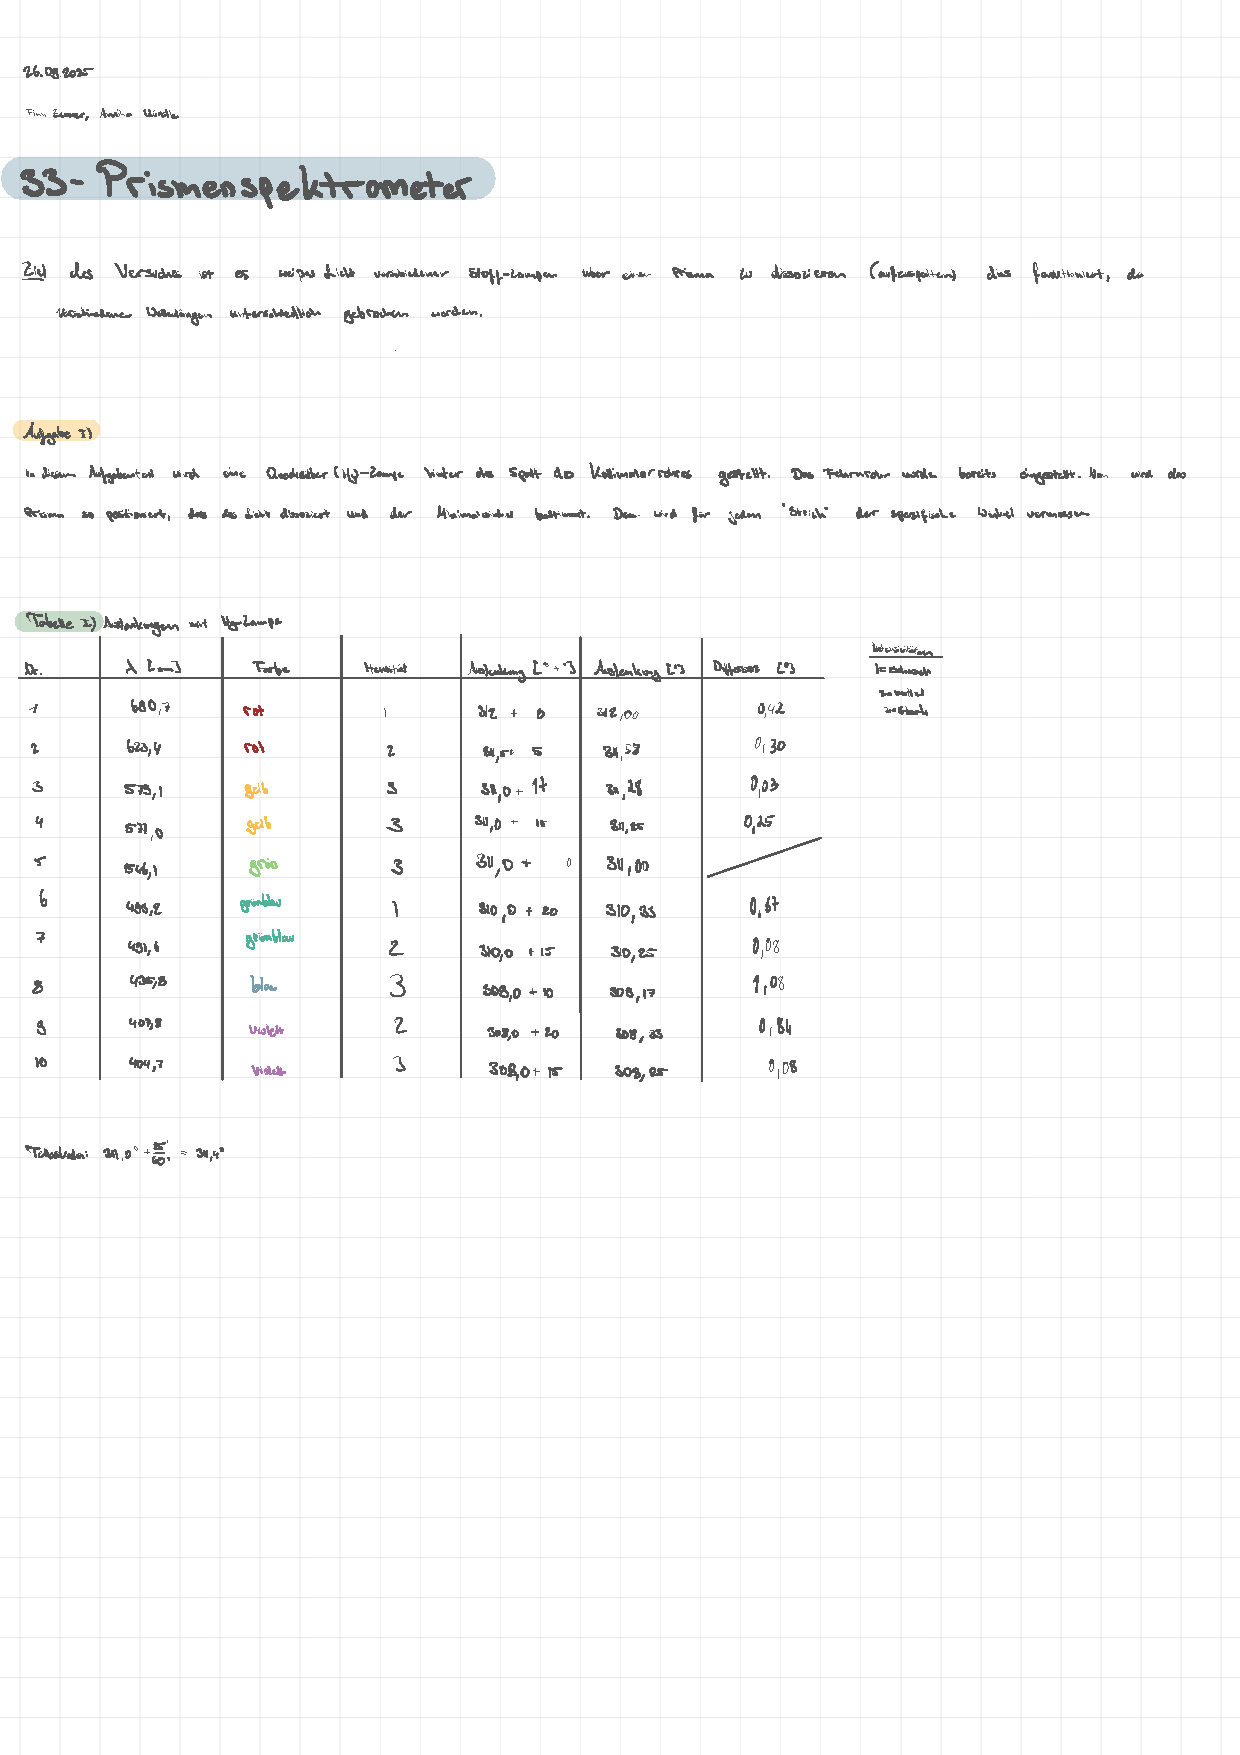
\includepdf[
  pages=1-3,               
  pagecommand={\thispagestyle{empty}} 
]{Protokolle/\versuchsnummer/Chapter/Messprotokoll.pdf}



\addcontentsline{lot}{table}{\protect\numberline{\thechapter.1} Messergebnisse der achromatisch korrigierten Linse}
\addcontentsline{lot}{table}{\protect\numberline{\thechapter.2} Besselverfahren für weißes Licht}
\addcontentsline{lot}{table}{\protect\numberline{\thechapter.3} Besselverfahren für rotes Licht}
\addcontentsline{lot}{table}{\protect\numberline{\thechapter.4} Besselverfahren für blaues Licht}
\addcontentsline{lot}{table}{\protect\numberline{\thechapter.5} Spaltbreiten}